\documentclass[10pt, compress, aspectratio=169]{beamer}

\usetheme[numbering=fraction, progressbar=none, titleformat=smallcaps]{metropolis}
\usepackage{booktabs}
\usepackage{array}
\usepackage{listings}
\usepackage{graphicx}
\usepackage[scale=2]{ccicons}
\usepackage{url}
\usepackage{relsize}
\usepackage{wasysym}

\usepackage{pgfplots}
\usepgfplotslibrary{dateplot}

\lstset{ %
  backgroundcolor={},
  basicstyle=\ttfamily\footnotesize,
  breakatwhitespace=true,
  breaklines=true,
  captionpos=n,
  commentstyle=\color{orange},
  escapeinside={\%*}{*)},
  extendedchars=true,
  frame=n,
  keywordstyle=\color{orange},
  language=C++,
  rulecolor=\color{black},
  showspaces=false,
  showstringspaces=false,
  showtabs=false,
  stepnumber=2,
  stringstyle=\color{gray},
  tabsize=2,
  keywords={thrust,plus,device_vector, copy,transform,begin,end, copyin,
  copyout, acc, \_\_global\_\_, void, int, float, main, threadIdx, blockIdx,
  blockDim, if, else, malloc, NULL, cudaMalloc, cudaMemcpy, cudaSuccess,
  cudaGetLastError, cudaDeviceSynchronize, cudaFree, cudaMemcpyDeviceToHost,
  cudaMemcpyHostToDevice, const, data, independent, kernels, loop,
  fprintf, stderr, cudaGetErrorString, EXIT_FAILURE, for, dim3},
  otherkeywords={::, \#pragma, \#include, <<<,>>>, \&, \*, +, -, /, [, ], >, <}
}

\renewcommand*{\UrlFont}{\ttfamily\smaller\relax}

\graphicspath{{images/}}

\title{Schedules}
\author{\footnotesize Rodrigo Siqueira \\ {\scriptsize siqueira@ime.usp.br}}
\institute{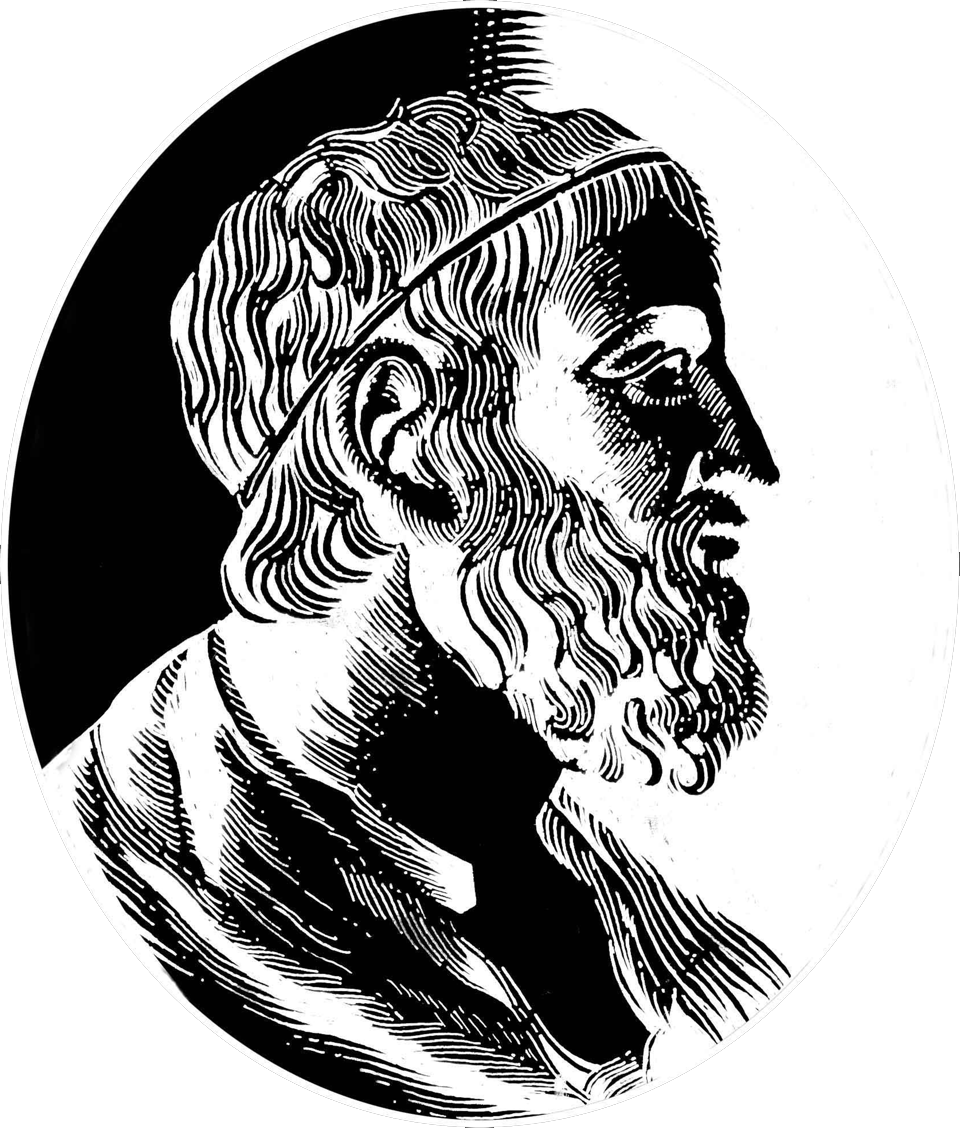
\includegraphics[height=2cm]{imelogo}\\[0.2cm] Department of Computer Science \\ University of São Paulo}

\begin{document}

\maketitle

%------------------------------------------------------------------------------
\section{Introduction}
\begin{frame}{Why use scheduler}
  \begin{itemize}
    \item Computers...
  \end{itemize}
\end{frame}

%------------------------------------------------------------------------------
\section{First-Come, First-Served (FCFS)}
\begin{frame}{An example from real life}
  % TODO: Create an image in upper view of many lines in the supermarket, use a
  % bunch of those image to explain the concept
  \begin{figure}[ht]
    \centering
    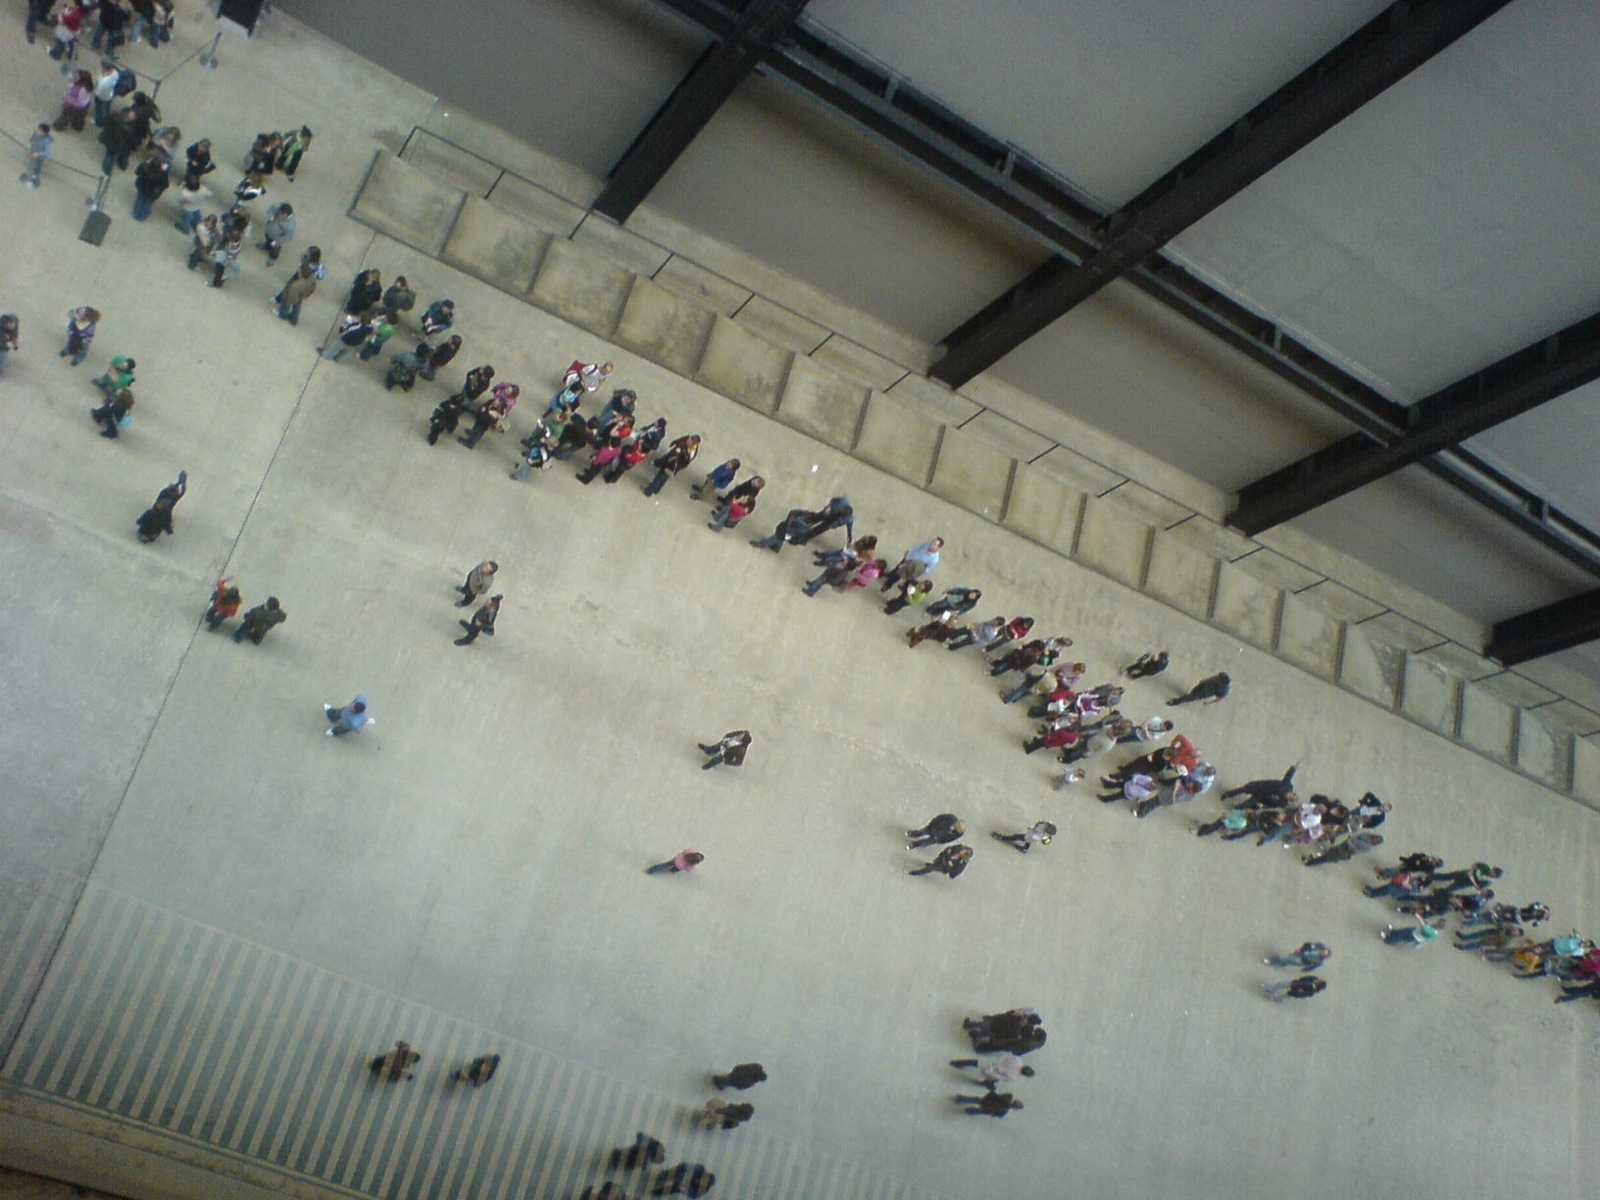
\includegraphics[width=0.7\textwidth, keepaspectratio=true]{images/fcfs.jpg}
  \end{figure}
\end{frame}

\begin{frame}{Fairness}
  % TODO: Create your own fairness icon

  \begin{columns}[T]
    \begin{column}{.5\textwidth}
      \begin{figure}[ht]
        \centering
        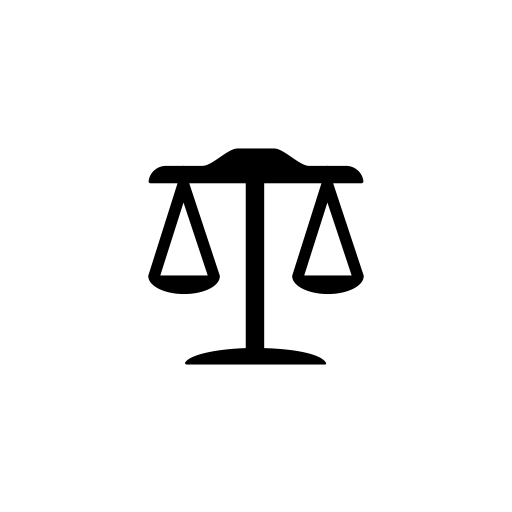
\includegraphics[width=0.6\textwidth, keepaspectratio=true]{images/fairness.png}
      \end{figure}
    \end{column}

    \hfill
    \begin{column}{.5\textwidth}
      \begin{itemize}
        \item Treat all equally
        \item Virtual line
      \end{itemize}
    \end{column}
  \end{columns}

\end{frame}

%------------------------------------------------------------------------------
\section{Shortest-job-first - SJF}
\begin{frame}{An example from real life}
  % TODO: Create some kind a HQ illustrating the situation of a guy that try
  % to full of water his bottle (drinking fountain)
  \begin{figure}[ht]
    \centering
    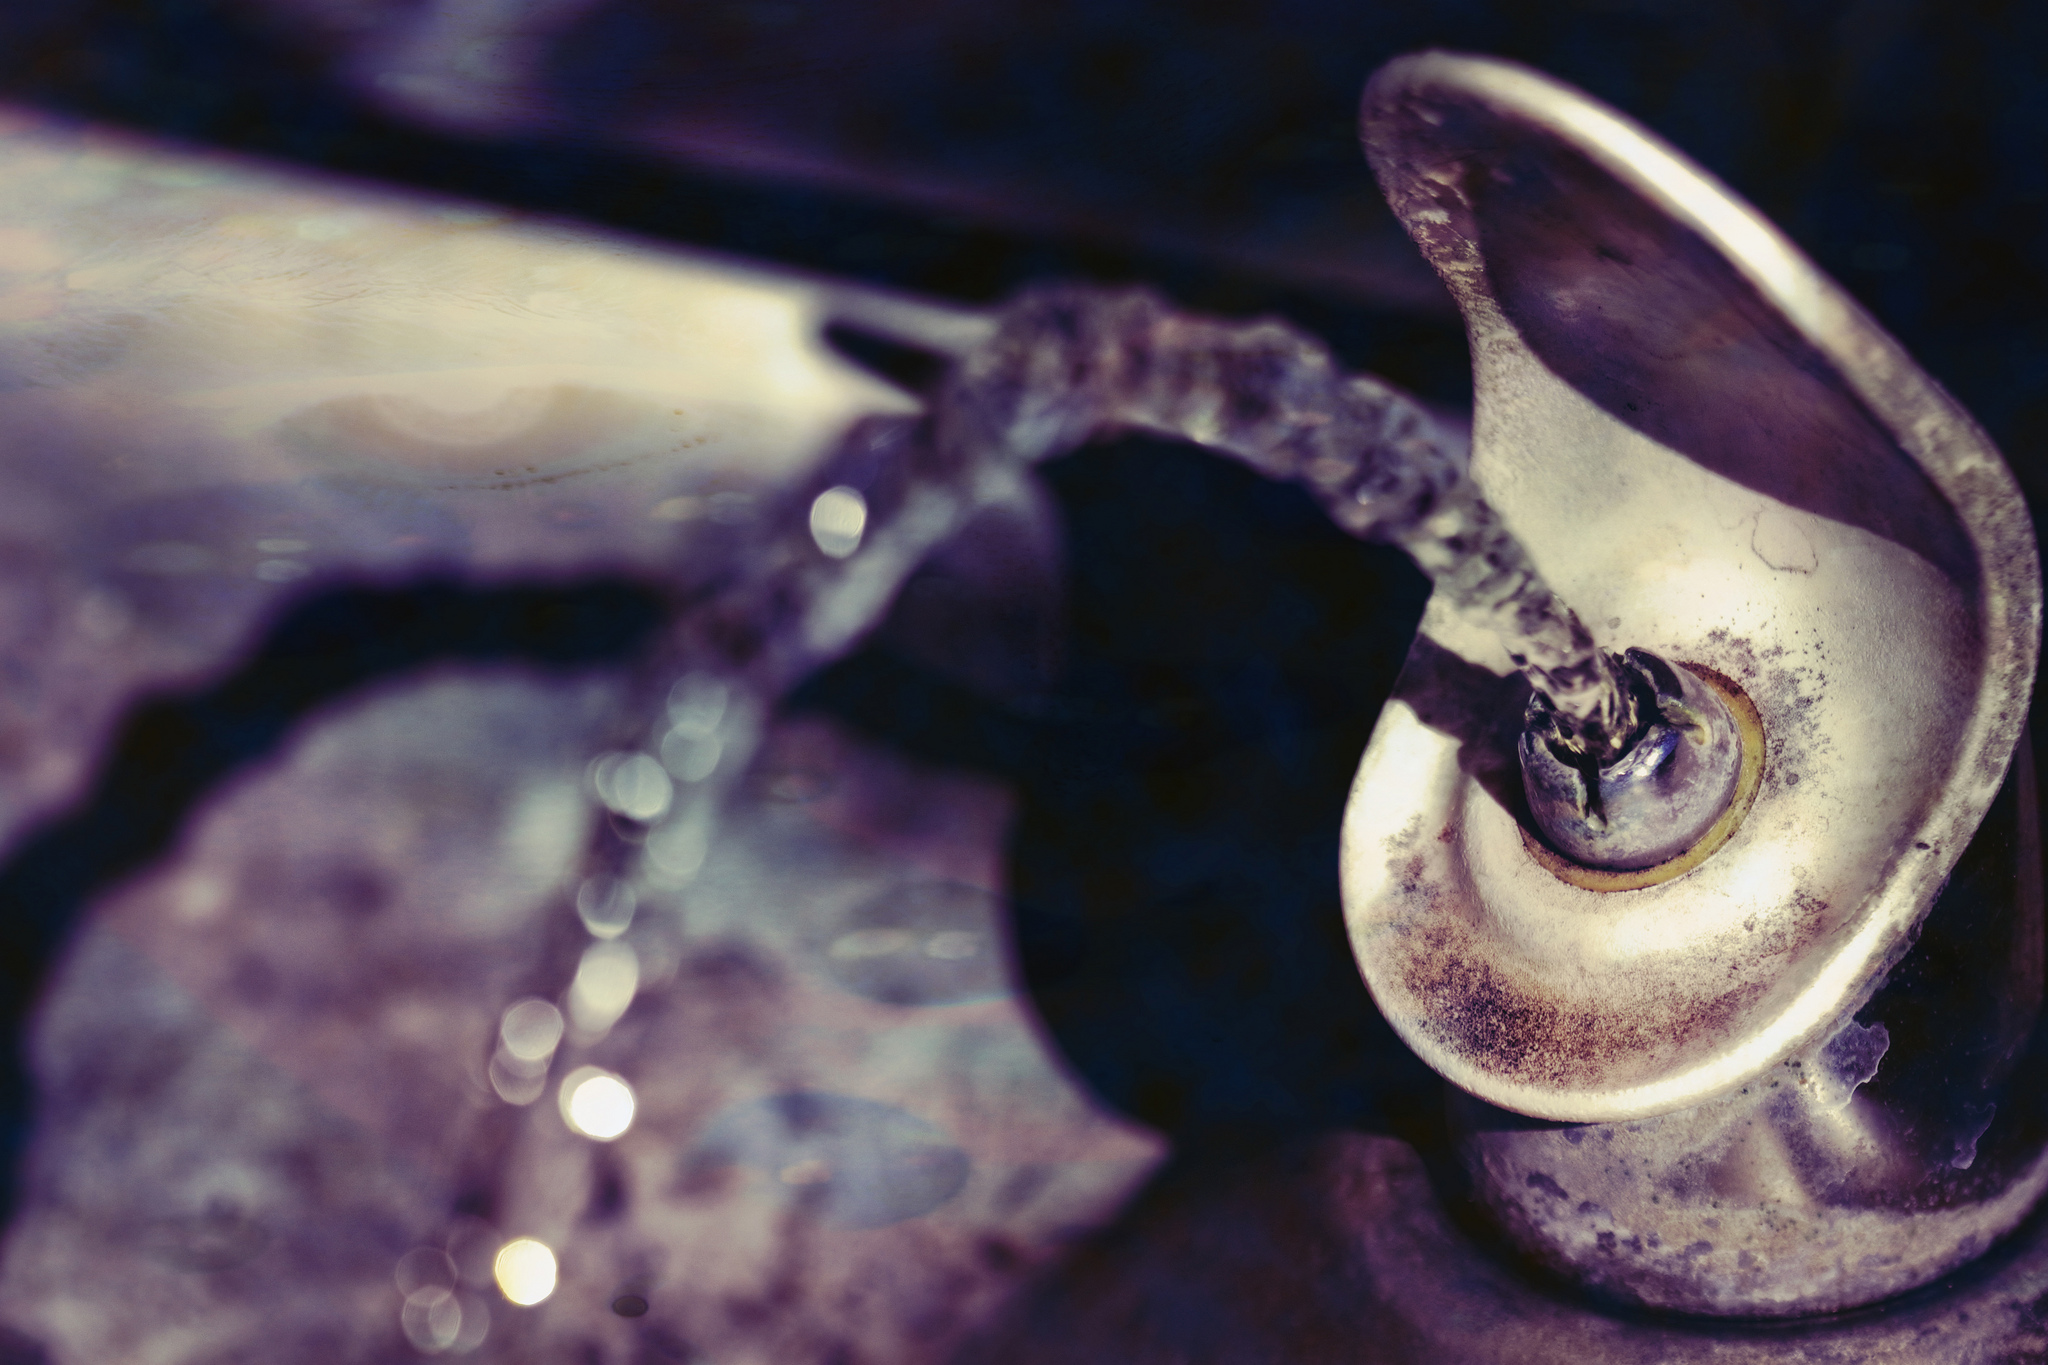
\includegraphics[width=0.7\textwidth, keepaspectratio=true]{images/sjf.jpg}
  \end{figure}
\end{frame}

\begin{frame}{Fairness on SJF}
  % TODO: Create your own fairness icon

  \begin{columns}[T]
    \begin{column}{.5\textwidth}
      \begin{figure}[ht]
        \centering
        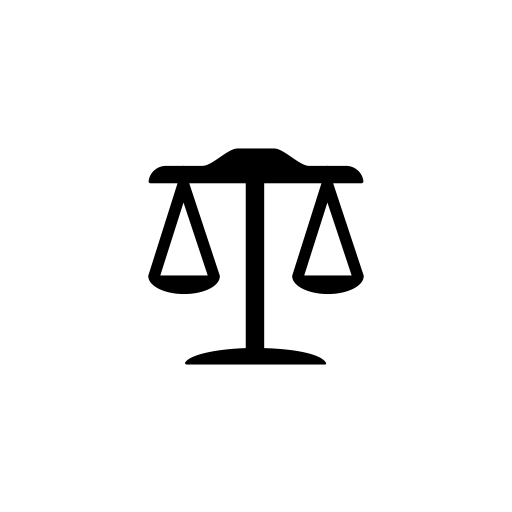
\includegraphics[width=0.6\textwidth, keepaspectratio=true]{images/fairness.png}
      \end{figure}
    \end{column}

    \hfill
    \begin{column}{.5\textwidth}
      \begin{itemize}
        \item Average waiting time
        \item Lower avarage
      \end{itemize}
    \end{column}
  \end{columns}

\end{frame}

%------------------------------------------------------------------------------
\section{Highest-Response-Ration-Next (HRRN)}
\begin{frame}{An example from real life}
  % TODO: Thinking a better image
  \begin{figure}[ht]
    \centering
    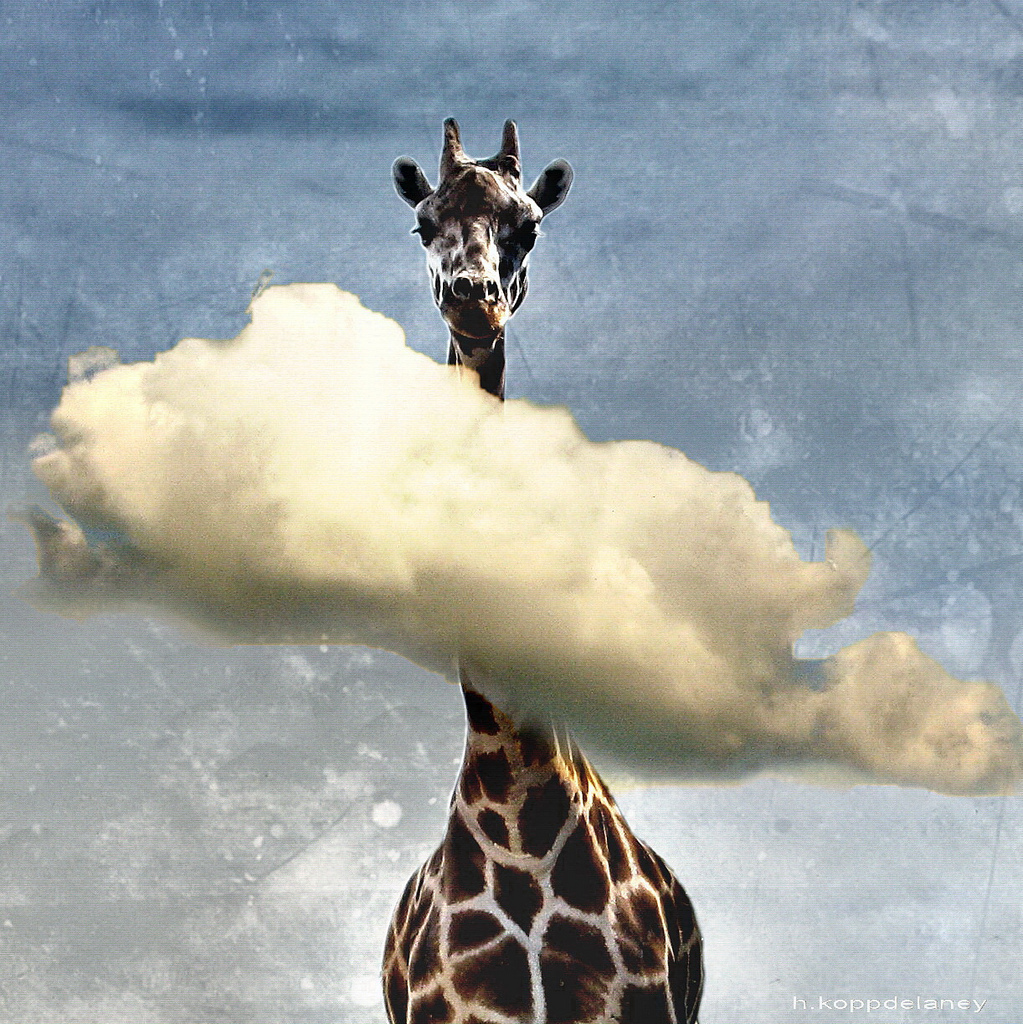
\includegraphics[width=0.7\textwidth, keepaspectratio=true]{images/hrrn.jpg}
  \end{figure}
\end{frame}

\begin{frame}{Fairness on HRRN}
  \begin{itemize}
    \item Problem with SJF
  \end{itemize}
\end{frame}

\begin{frame}{Fairness on HRRN}
  % TODO: Create your own fairness icon

  \begin{columns}[T]
    \begin{column}{.4\textwidth}
      \begin{figure}[ht]
        \centering
        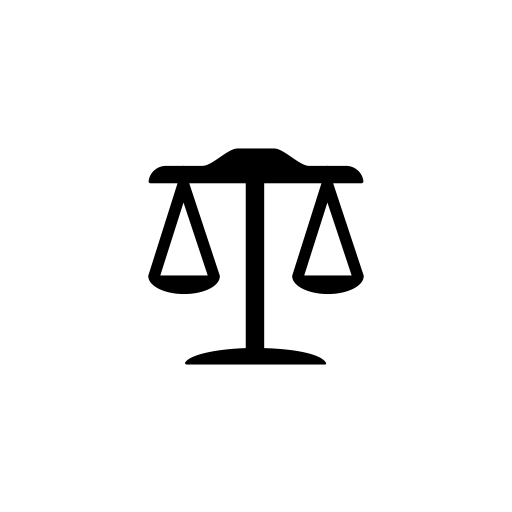
\includegraphics[width=0.6\textwidth, keepaspectratio=true]{images/fairness.png}
      \end{figure}
    \end{column}

    \hfill
    \begin{column}{.6\textwidth}
      \begin{itemize}
        \item Reduce the waiting time for long jobs
      \end{itemize}

      \begin{equation*}
         responseRate = \frac{waitingTime + wastTime}{waitingTime}
      \end{equation*}
    \end{column}
  \end{columns}

\end{frame}

%------------------------------------------------------------------------------
\section{Round-Robin (RR)}
\begin{frame}{An example from real life}
  % TODO: Create some kind of cartoon to illustrate this idea
  \begin{figure}[ht]
    \centering
    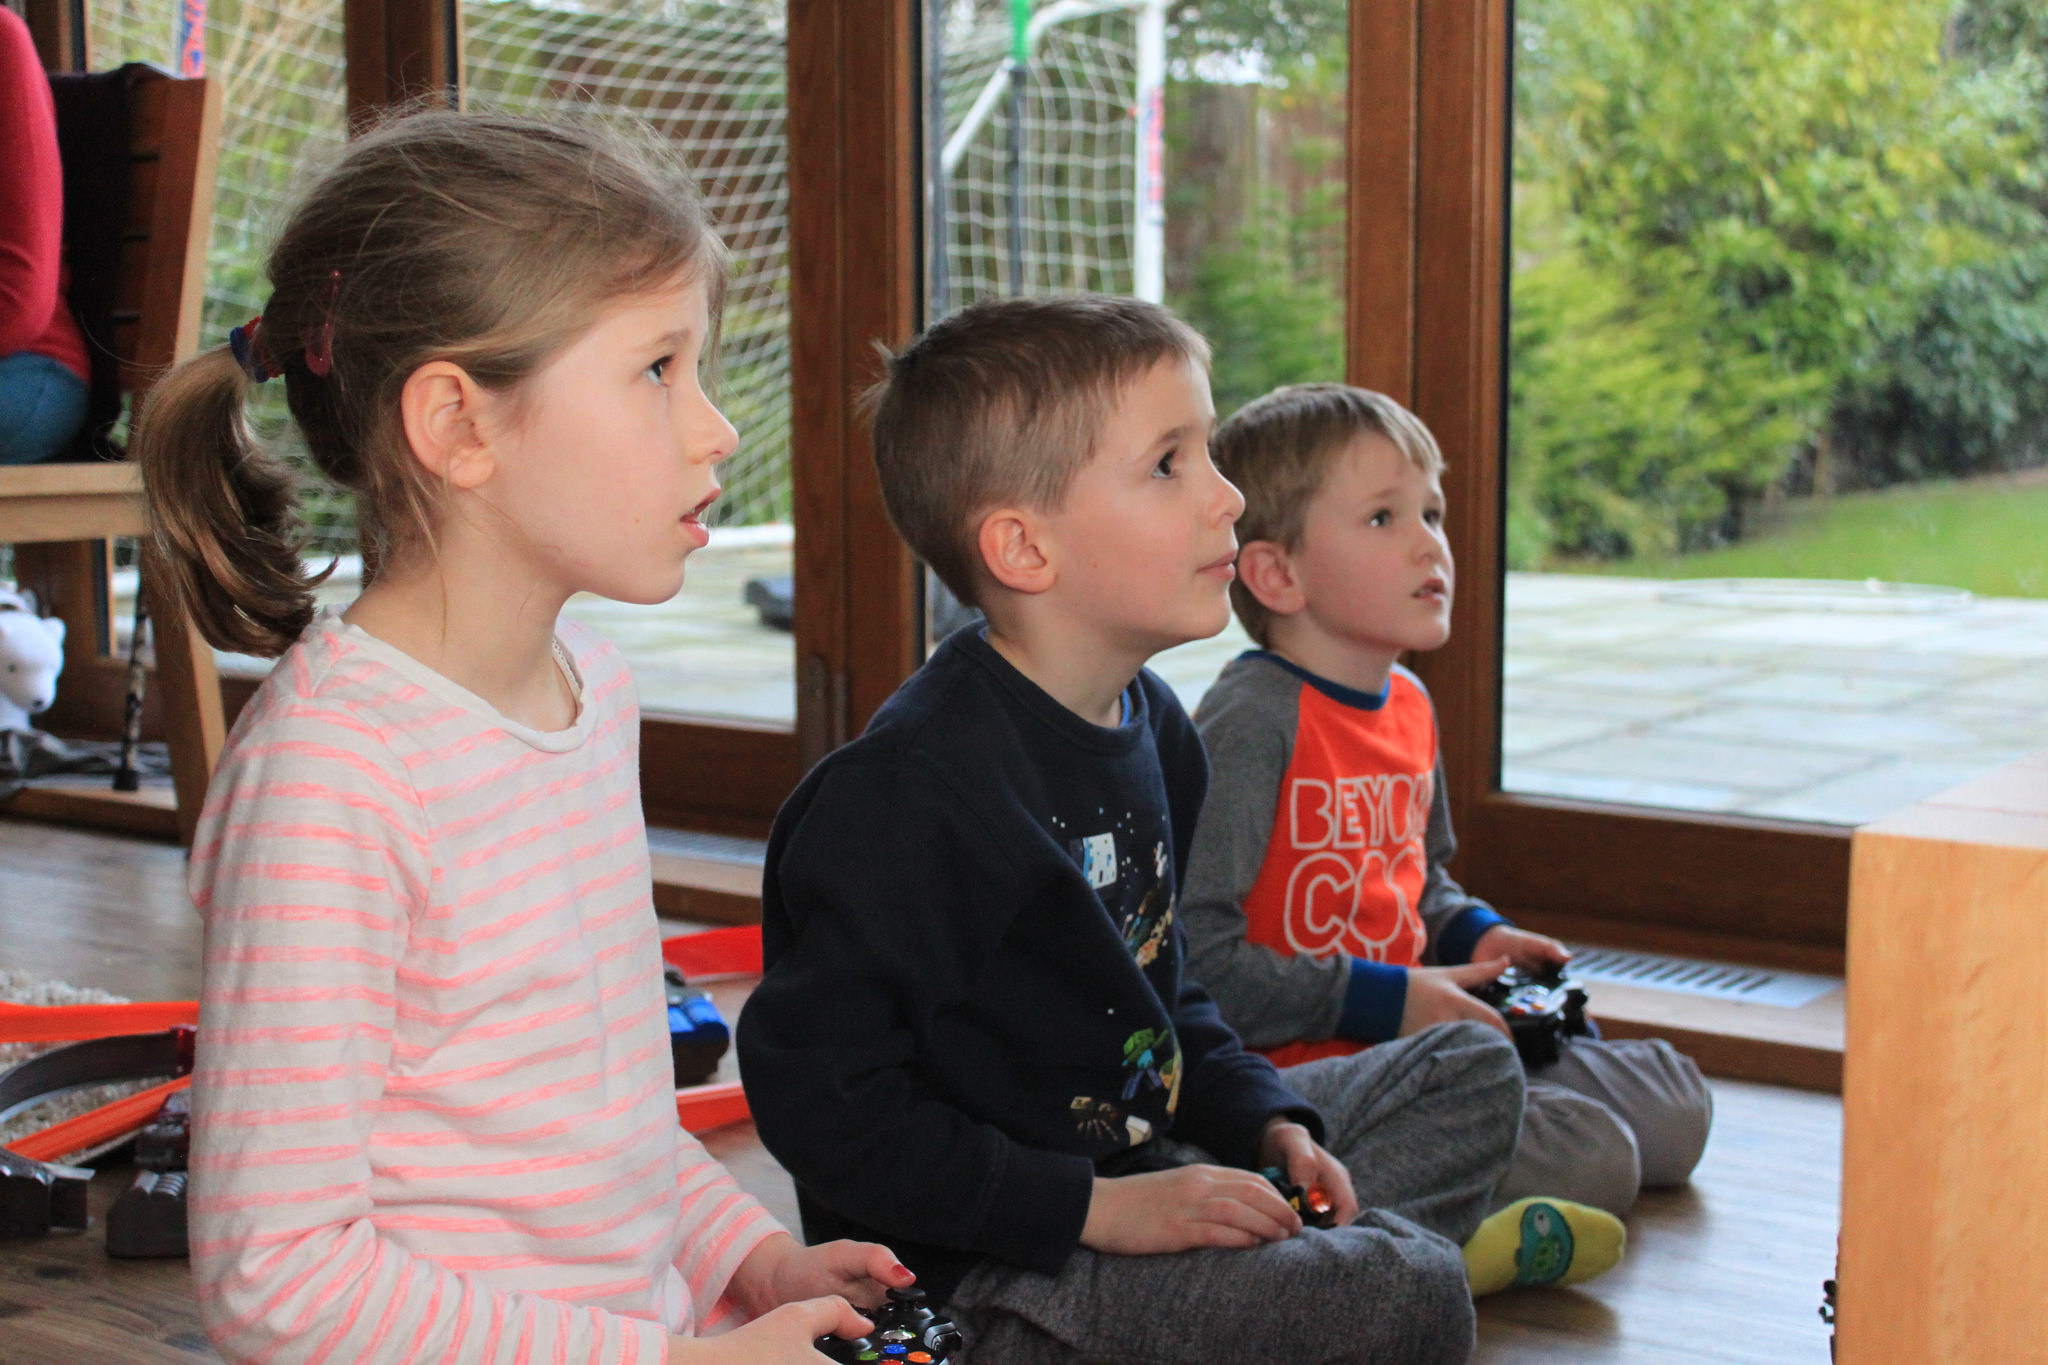
\includegraphics[width=0.7\textwidth, keepaspectratio=true]{images/play_video_game.jpg}
  \end{figure}
\end{frame}

\begin{frame}{How it works?}
  % TODO: Create the control flow of this algorithm
  \begin{itemize}
    \item Preemption
    \item Time-slice
    \item Stop to execute
    \item Waiting queue for I/O
  \end{itemize}
\end{frame}

\begin{frame}{Quantum/time-slice}
  % TODO: Create the control flow of this algorithm
  \begin{itemize}
    \item How to choose a quantum size?
    \item Long quantum Vs Short quantum
    \item Iteratively size define
  \end{itemize}
\end{frame}

%------------------------------------------------------------------------------
\section{Multiple queues}
\begin{frame}{How it works?}
  % TODO: Create some kind of cartoon to illustrate this idea
  \begin{itemize}
    \item Example with one queue
    \item Example with multiple queue
  \end{itemize}
\end{frame}

%------------------------------------------------------------------------------
\section{Political Vs Mechanism}
\begin{frame}{What is the difference}
  % TODO: Create some slides to this
\end{frame}

%------------------------------------------------------------------------------
\section{About this presentation}
\begin{frame}[standout]
  % TODO: Improve it
   \begin{center}\ccbysa\end{center}
\end{frame}


\maketitle

\end{document}
